\PassOptionsToPackage{unicode=true}{hyperref} % options for packages loaded elsewhere
\PassOptionsToPackage{hyphens}{url}
%
\documentclass[]{article}
\usepackage{lmodern}
\usepackage{amssymb,amsmath}
\usepackage{ifxetex,ifluatex}
\usepackage{fixltx2e} % provides \textsubscript
\ifnum 0\ifxetex 1\fi\ifluatex 1\fi=0 % if pdftex
  \usepackage[T1]{fontenc}
  \usepackage[utf8]{inputenc}
  \usepackage{textcomp} % provides euro and other symbols
\else % if luatex or xelatex
  \usepackage{unicode-math}
  \defaultfontfeatures{Ligatures=TeX,Scale=MatchLowercase}
\fi
% use upquote if available, for straight quotes in verbatim environments
\IfFileExists{upquote.sty}{\usepackage{upquote}}{}
% use microtype if available
\IfFileExists{microtype.sty}{%
\usepackage[]{microtype}
\UseMicrotypeSet[protrusion]{basicmath} % disable protrusion for tt fonts
}{}
\IfFileExists{parskip.sty}{%
\usepackage{parskip}
}{% else
\setlength{\parindent}{0pt}
\setlength{\parskip}{6pt plus 2pt minus 1pt}
}
\usepackage{hyperref}
\hypersetup{
            pdftitle={Final Report},
            pdfauthor={Carleena Ortega and Saelin Bjornson},
            pdfborder={0 0 0},
            breaklinks=true}
\urlstyle{same}  % don't use monospace font for urls
\usepackage[margin=1in]{geometry}
\usepackage{color}
\usepackage{fancyvrb}
\newcommand{\VerbBar}{|}
\newcommand{\VERB}{\Verb[commandchars=\\\{\}]}
\DefineVerbatimEnvironment{Highlighting}{Verbatim}{commandchars=\\\{\}}
% Add ',fontsize=\small' for more characters per line
\usepackage{framed}
\definecolor{shadecolor}{RGB}{248,248,248}
\newenvironment{Shaded}{\begin{snugshade}}{\end{snugshade}}
\newcommand{\AlertTok}[1]{\textcolor[rgb]{0.94,0.16,0.16}{#1}}
\newcommand{\AnnotationTok}[1]{\textcolor[rgb]{0.56,0.35,0.01}{\textbf{\textit{#1}}}}
\newcommand{\AttributeTok}[1]{\textcolor[rgb]{0.77,0.63,0.00}{#1}}
\newcommand{\BaseNTok}[1]{\textcolor[rgb]{0.00,0.00,0.81}{#1}}
\newcommand{\BuiltInTok}[1]{#1}
\newcommand{\CharTok}[1]{\textcolor[rgb]{0.31,0.60,0.02}{#1}}
\newcommand{\CommentTok}[1]{\textcolor[rgb]{0.56,0.35,0.01}{\textit{#1}}}
\newcommand{\CommentVarTok}[1]{\textcolor[rgb]{0.56,0.35,0.01}{\textbf{\textit{#1}}}}
\newcommand{\ConstantTok}[1]{\textcolor[rgb]{0.00,0.00,0.00}{#1}}
\newcommand{\ControlFlowTok}[1]{\textcolor[rgb]{0.13,0.29,0.53}{\textbf{#1}}}
\newcommand{\DataTypeTok}[1]{\textcolor[rgb]{0.13,0.29,0.53}{#1}}
\newcommand{\DecValTok}[1]{\textcolor[rgb]{0.00,0.00,0.81}{#1}}
\newcommand{\DocumentationTok}[1]{\textcolor[rgb]{0.56,0.35,0.01}{\textbf{\textit{#1}}}}
\newcommand{\ErrorTok}[1]{\textcolor[rgb]{0.64,0.00,0.00}{\textbf{#1}}}
\newcommand{\ExtensionTok}[1]{#1}
\newcommand{\FloatTok}[1]{\textcolor[rgb]{0.00,0.00,0.81}{#1}}
\newcommand{\FunctionTok}[1]{\textcolor[rgb]{0.00,0.00,0.00}{#1}}
\newcommand{\ImportTok}[1]{#1}
\newcommand{\InformationTok}[1]{\textcolor[rgb]{0.56,0.35,0.01}{\textbf{\textit{#1}}}}
\newcommand{\KeywordTok}[1]{\textcolor[rgb]{0.13,0.29,0.53}{\textbf{#1}}}
\newcommand{\NormalTok}[1]{#1}
\newcommand{\OperatorTok}[1]{\textcolor[rgb]{0.81,0.36,0.00}{\textbf{#1}}}
\newcommand{\OtherTok}[1]{\textcolor[rgb]{0.56,0.35,0.01}{#1}}
\newcommand{\PreprocessorTok}[1]{\textcolor[rgb]{0.56,0.35,0.01}{\textit{#1}}}
\newcommand{\RegionMarkerTok}[1]{#1}
\newcommand{\SpecialCharTok}[1]{\textcolor[rgb]{0.00,0.00,0.00}{#1}}
\newcommand{\SpecialStringTok}[1]{\textcolor[rgb]{0.31,0.60,0.02}{#1}}
\newcommand{\StringTok}[1]{\textcolor[rgb]{0.31,0.60,0.02}{#1}}
\newcommand{\VariableTok}[1]{\textcolor[rgb]{0.00,0.00,0.00}{#1}}
\newcommand{\VerbatimStringTok}[1]{\textcolor[rgb]{0.31,0.60,0.02}{#1}}
\newcommand{\WarningTok}[1]{\textcolor[rgb]{0.56,0.35,0.01}{\textbf{\textit{#1}}}}
\usepackage{longtable,booktabs}
% Fix footnotes in tables (requires footnote package)
\IfFileExists{footnote.sty}{\usepackage{footnote}\makesavenoteenv{longtable}}{}
\usepackage{graphicx,grffile}
\makeatletter
\def\maxwidth{\ifdim\Gin@nat@width>\linewidth\linewidth\else\Gin@nat@width\fi}
\def\maxheight{\ifdim\Gin@nat@height>\textheight\textheight\else\Gin@nat@height\fi}
\makeatother
% Scale images if necessary, so that they will not overflow the page
% margins by default, and it is still possible to overwrite the defaults
% using explicit options in \includegraphics[width, height, ...]{}
\setkeys{Gin}{width=\maxwidth,height=\maxheight,keepaspectratio}
\setlength{\emergencystretch}{3em}  % prevent overfull lines
\providecommand{\tightlist}{%
  \setlength{\itemsep}{0pt}\setlength{\parskip}{0pt}}
\setcounter{secnumdepth}{0}
% Redefines (sub)paragraphs to behave more like sections
\ifx\paragraph\undefined\else
\let\oldparagraph\paragraph
\renewcommand{\paragraph}[1]{\oldparagraph{#1}\mbox{}}
\fi
\ifx\subparagraph\undefined\else
\let\oldsubparagraph\subparagraph
\renewcommand{\subparagraph}[1]{\oldsubparagraph{#1}\mbox{}}
\fi

% set default figure placement to htbp
\makeatletter
\def\fps@figure{htbp}
\makeatother

\usepackage{booktabs}
\usepackage{longtable}
\usepackage{array}
\usepackage{multirow}
\usepackage{wrapfig}
\usepackage{float}
\usepackage{colortbl}
\usepackage{pdflscape}
\usepackage{tabu}
\usepackage{threeparttable}
\usepackage{threeparttablex}
\usepackage[normalem]{ulem}
\usepackage{makecell}
\usepackage{xcolor}

\title{Final Report}
\author{Carleena Ortega and Saelin Bjornson}
\date{15/03/2020}

\begin{document}
\maketitle

{
\setcounter{tocdepth}{4}
\tableofcontents
}
\hypertarget{adult-income}{%
\subsection{Adult Income}\label{adult-income}}

\hypertarget{introduction}{%
\subsection{Introduction}\label{introduction}}

\hypertarget{the-dataset}{%
\subsubsection{The Dataset}\label{the-dataset}}

Who: The data set was extracted by Barry Becker from the 1994 Census
database and is donated by Silicon Graphics\\
What: This is a multivariate dataset with categorical and integer
variables. It contains the predicted income of individuals from the
census with attributes including age, marital status, work class,
education, sex, and race.\\
When: The data is from a 1994 census.\\
Why: The data set is found in the University of California Irvine
Machine Learning Repository, and was used for ML prediction of whether a
person makes over or under 50K a year based on their attributes.\\
How: The census data was collected by survey.

\hypertarget{the-variables}{%
\subsubsection{The Variables}\label{the-variables}}

\begin{longtable}[]{@{}lll@{}}
\toprule
\begin{minipage}[b]{0.35\columnwidth}\raggedright
Variable\strut
\end{minipage} & \begin{minipage}[b]{0.30\columnwidth}\raggedright
Type\strut
\end{minipage} & \begin{minipage}[b]{0.26\columnwidth}\raggedright
Description\strut
\end{minipage}\tabularnewline
\midrule
\endhead
\begin{minipage}[t]{0.35\columnwidth}\raggedright
age\strut
\end{minipage} & \begin{minipage}[t]{0.30\columnwidth}\raggedright
int\strut
\end{minipage} & \begin{minipage}[t]{0.26\columnwidth}\raggedright
Age of individual\strut
\end{minipage}\tabularnewline
\begin{minipage}[t]{0.35\columnwidth}\raggedright
workclass\strut
\end{minipage} & \begin{minipage}[t]{0.30\columnwidth}\raggedright
chr\strut
\end{minipage} & \begin{minipage}[t]{0.26\columnwidth}\raggedright
e.g.~private, self-emplowed, federal government, never worked,
etc.\strut
\end{minipage}\tabularnewline
\begin{minipage}[t]{0.35\columnwidth}\raggedright
fnlwgt\strut
\end{minipage} & \begin{minipage}[t]{0.30\columnwidth}\raggedright
int\strut
\end{minipage} & \begin{minipage}[t]{0.26\columnwidth}\raggedright
Final weights: weighted sums of the socio-economic characteristics of
the individual. People with similar demographics have similar
weights.\strut
\end{minipage}\tabularnewline
\begin{minipage}[t]{0.35\columnwidth}\raggedright
education\strut
\end{minipage} & \begin{minipage}[t]{0.30\columnwidth}\raggedright
chr\strut
\end{minipage} & \begin{minipage}[t]{0.26\columnwidth}\raggedright
Highest education recieved\strut
\end{minipage}\tabularnewline
\begin{minipage}[t]{0.35\columnwidth}\raggedright
educationnum\strut
\end{minipage} & \begin{minipage}[t]{0.30\columnwidth}\raggedright
factor\strut
\end{minipage} & \begin{minipage}[t]{0.26\columnwidth}\raggedright
Numerical code for highest education recieved\strut
\end{minipage}\tabularnewline
\begin{minipage}[t]{0.35\columnwidth}\raggedright
marital\_status\strut
\end{minipage} & \begin{minipage}[t]{0.30\columnwidth}\raggedright
int\strut
\end{minipage} & \begin{minipage}[t]{0.26\columnwidth}\raggedright
e.g.~married, never married, divorced, etc.\strut
\end{minipage}\tabularnewline
\begin{minipage}[t]{0.35\columnwidth}\raggedright
occupation\strut
\end{minipage} & \begin{minipage}[t]{0.30\columnwidth}\raggedright
chr\strut
\end{minipage} & \begin{minipage}[t]{0.26\columnwidth}\raggedright
Occupation of individual\strut
\end{minipage}\tabularnewline
\begin{minipage}[t]{0.35\columnwidth}\raggedright
relationship\strut
\end{minipage} & \begin{minipage}[t]{0.30\columnwidth}\raggedright
chr\strut
\end{minipage} & \begin{minipage}[t]{0.26\columnwidth}\raggedright
Relation of individual in family. e.g.~wife, child, husband,
unmarried\strut
\end{minipage}\tabularnewline
\begin{minipage}[t]{0.35\columnwidth}\raggedright
race\strut
\end{minipage} & \begin{minipage}[t]{0.30\columnwidth}\raggedright
chr\strut
\end{minipage} & \begin{minipage}[t]{0.26\columnwidth}\raggedright
Asian-Pacific Islander, Native American, White, Black, other\strut
\end{minipage}\tabularnewline
\begin{minipage}[t]{0.35\columnwidth}\raggedright
sex\strut
\end{minipage} & \begin{minipage}[t]{0.30\columnwidth}\raggedright
chr\strut
\end{minipage} & \begin{minipage}[t]{0.26\columnwidth}\raggedright
Male or Female\strut
\end{minipage}\tabularnewline
\begin{minipage}[t]{0.35\columnwidth}\raggedright
capital\_gain\strut
\end{minipage} & \begin{minipage}[t]{0.30\columnwidth}\raggedright
int\strut
\end{minipage} & \begin{minipage}[t]{0.26\columnwidth}\raggedright
Profit from capital assets such as investments, real estate, etc.\strut
\end{minipage}\tabularnewline
\begin{minipage}[t]{0.35\columnwidth}\raggedright
capital\_loss\strut
\end{minipage} & \begin{minipage}[t]{0.30\columnwidth}\raggedright
int\strut
\end{minipage} & \begin{minipage}[t]{0.26\columnwidth}\raggedright
Loss from capital assets\strut
\end{minipage}\tabularnewline
\begin{minipage}[t]{0.35\columnwidth}\raggedright
hours\_per\_week\strut
\end{minipage} & \begin{minipage}[t]{0.30\columnwidth}\raggedright
\strut
\end{minipage} & \begin{minipage}[t]{0.26\columnwidth}\raggedright
The number of hours that the individual works per week\strut
\end{minipage}\tabularnewline
\begin{minipage}[t]{0.35\columnwidth}\raggedright
country\strut
\end{minipage} & \begin{minipage}[t]{0.30\columnwidth}\raggedright
chr\strut
\end{minipage} & \begin{minipage}[t]{0.26\columnwidth}\raggedright
Country of origin\strut
\end{minipage}\tabularnewline
\begin{minipage}[t]{0.35\columnwidth}\raggedright
income\strut
\end{minipage} & \begin{minipage}[t]{0.30\columnwidth}\raggedright
chr\strut
\end{minipage} & \begin{minipage}[t]{0.26\columnwidth}\raggedright
Whether individual is predicted to make over or under 50K\strut
\end{minipage}\tabularnewline
\bottomrule
\end{longtable}

The single group used in the following analysis includes divorced,
widowed, and never married individuals while the married group includes
individials currently married (whether separated, together, or etc.)

\hypertarget{the-research-question-and-method}{%
\subsubsection{The Research Question and
Method}\label{the-research-question-and-method}}

\textbf{Are the number of hours someone works per week correlated with
their age, relationship, education level, race or sex?}

Plots showing the relationship between hours worked and each variable
separately. For example, we will use the linear regression model to
explore how hours at work is related to variables such as age,
relationship, education level, and sex.

\hypertarget{exploratory-data-analysis}{%
\subsection{Exploratory Data Analysis}\label{exploratory-data-analysis}}

In this section, we will get to know our dataset better by exploring the
relationship between certain factors.

\hypertarget{age-and-sex}{%
\subsubsection{Age and Sex}\label{age-and-sex}}

The plot below shows that there are more male employees than female
employees and that the majority of working males are older than working
females since the male (blue curve) have a peak shifted to the right
with respect to female (red peak).

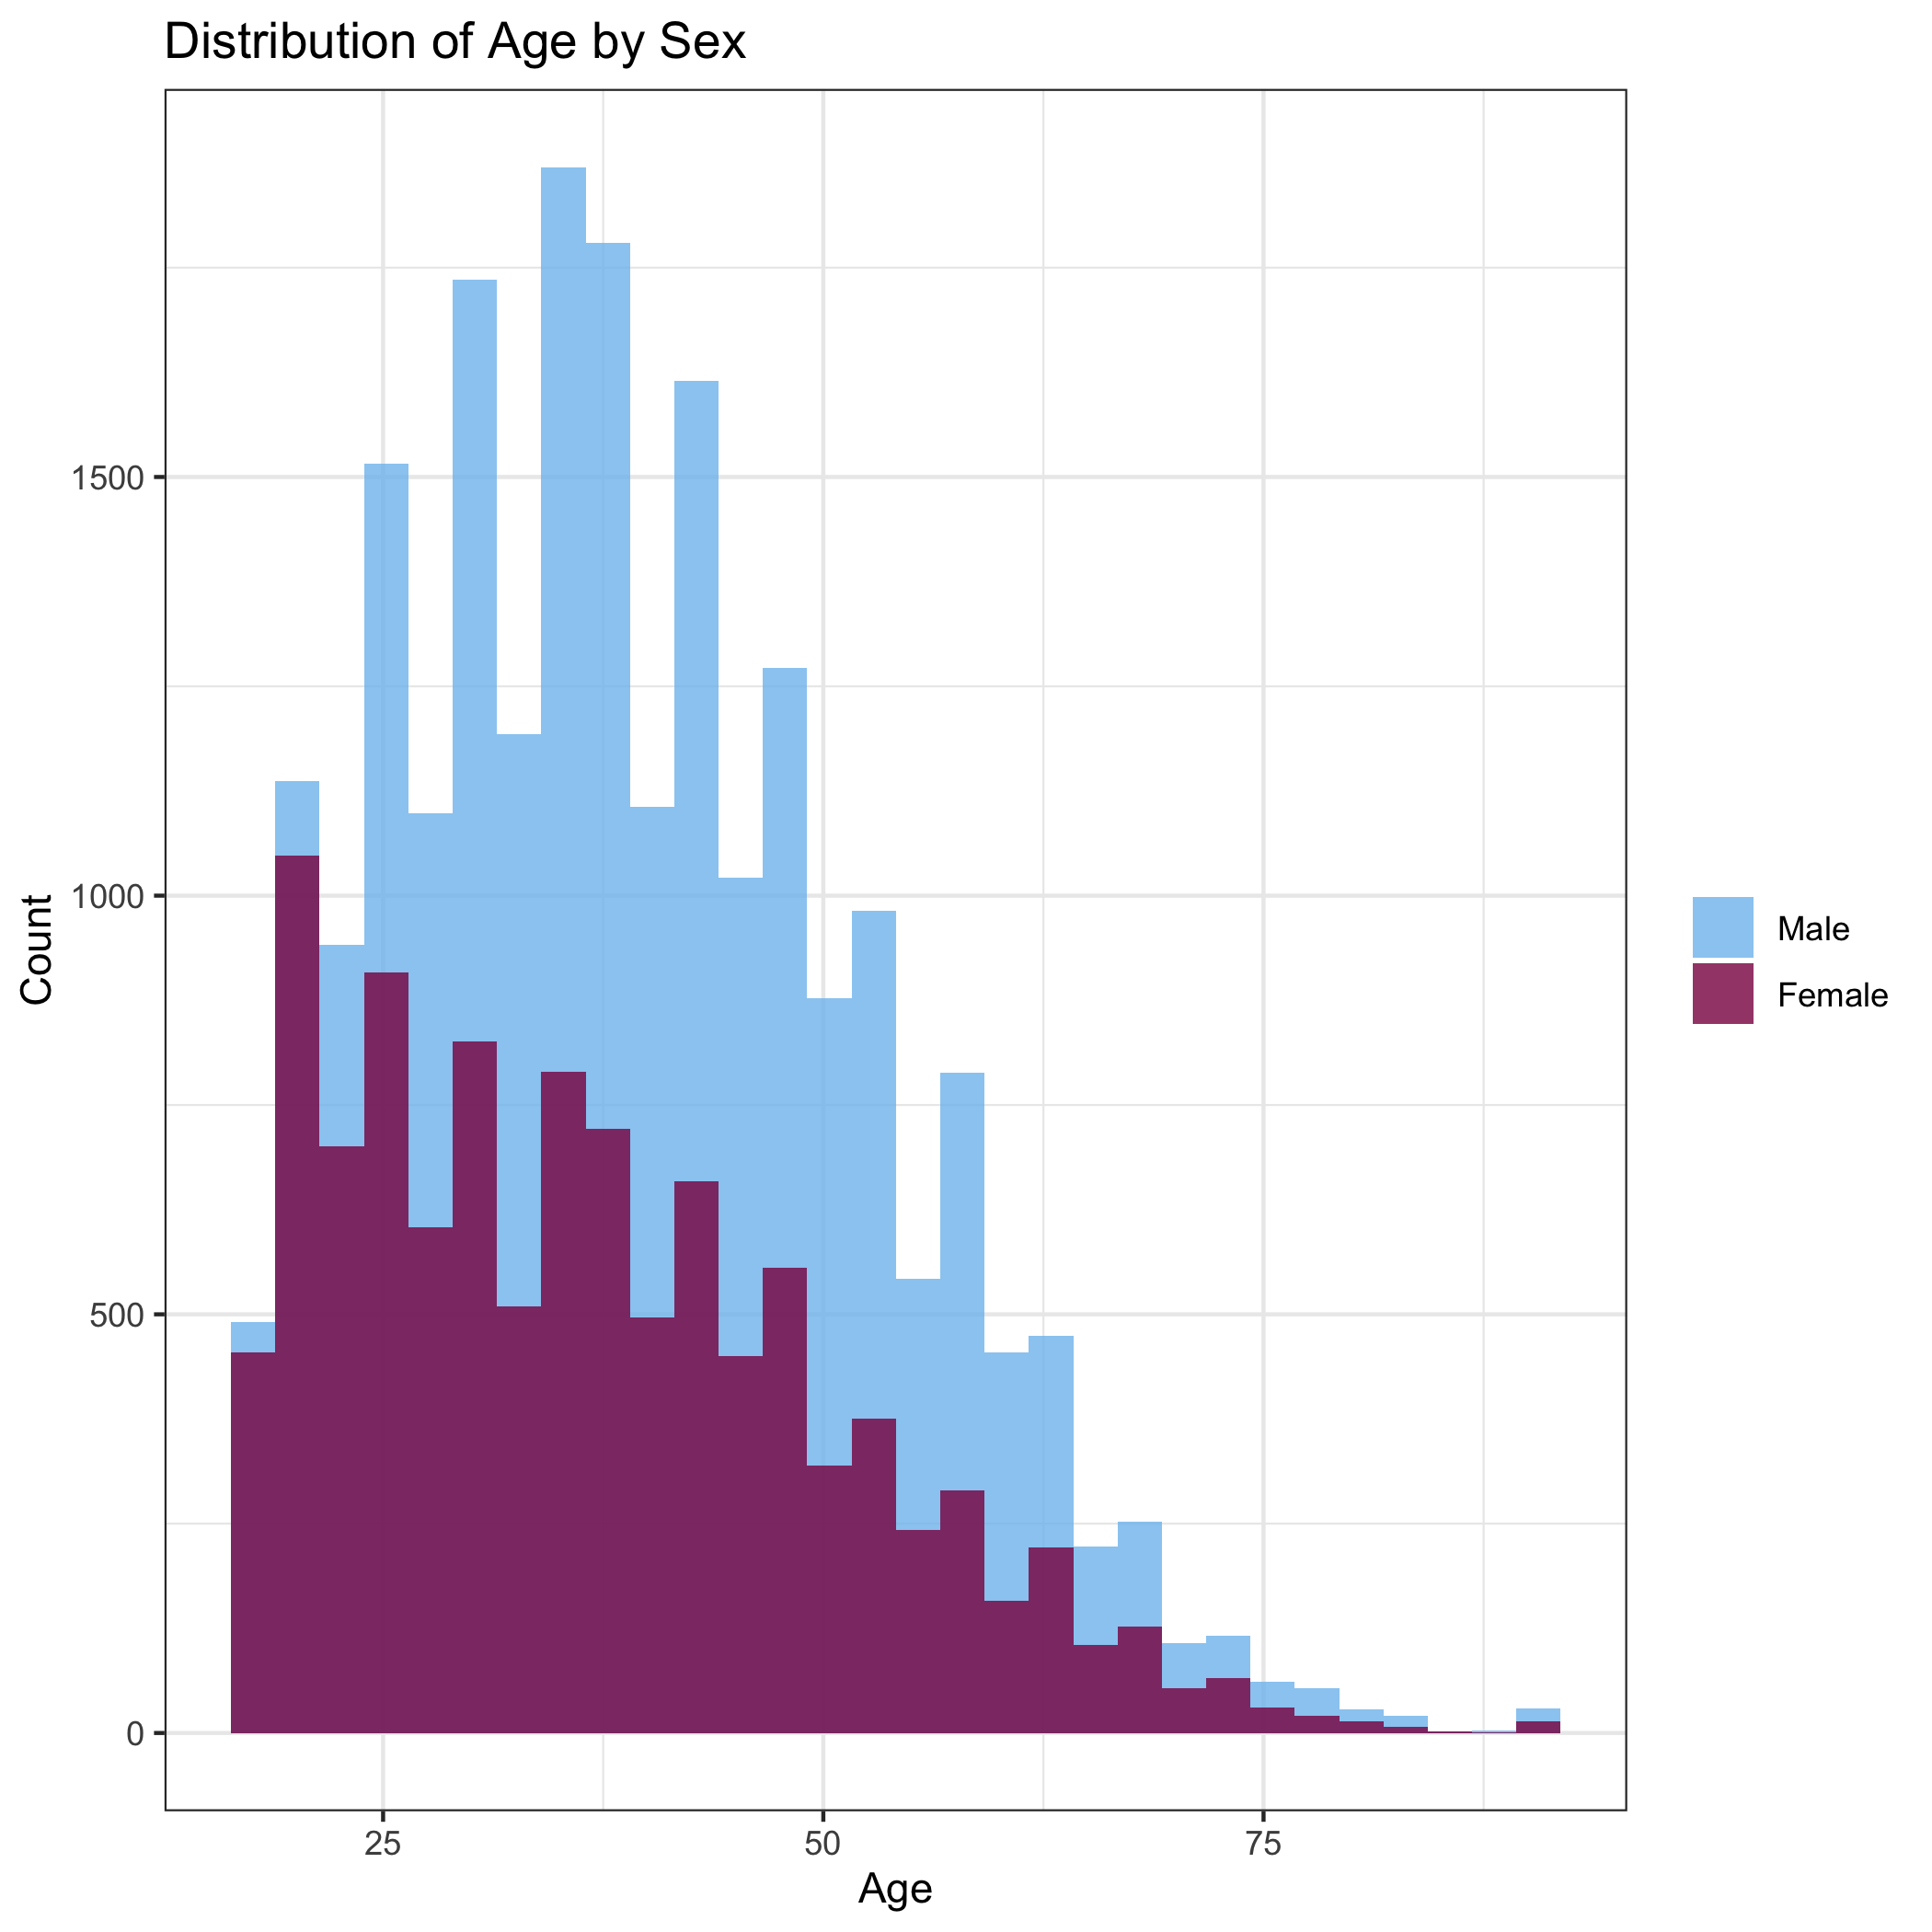
\includegraphics{../images/Plot_1_Distribution_of_Age_by_Sex.png}

\hypertarget{educational-level-and-income}{%
\subsubsection{Educational Level and
Income}\label{educational-level-and-income}}

We observe from the following graphs that a majority of individuals
earning greater than \$50,000 a year only accomplished high school
irrespective of sex or ethnical background.

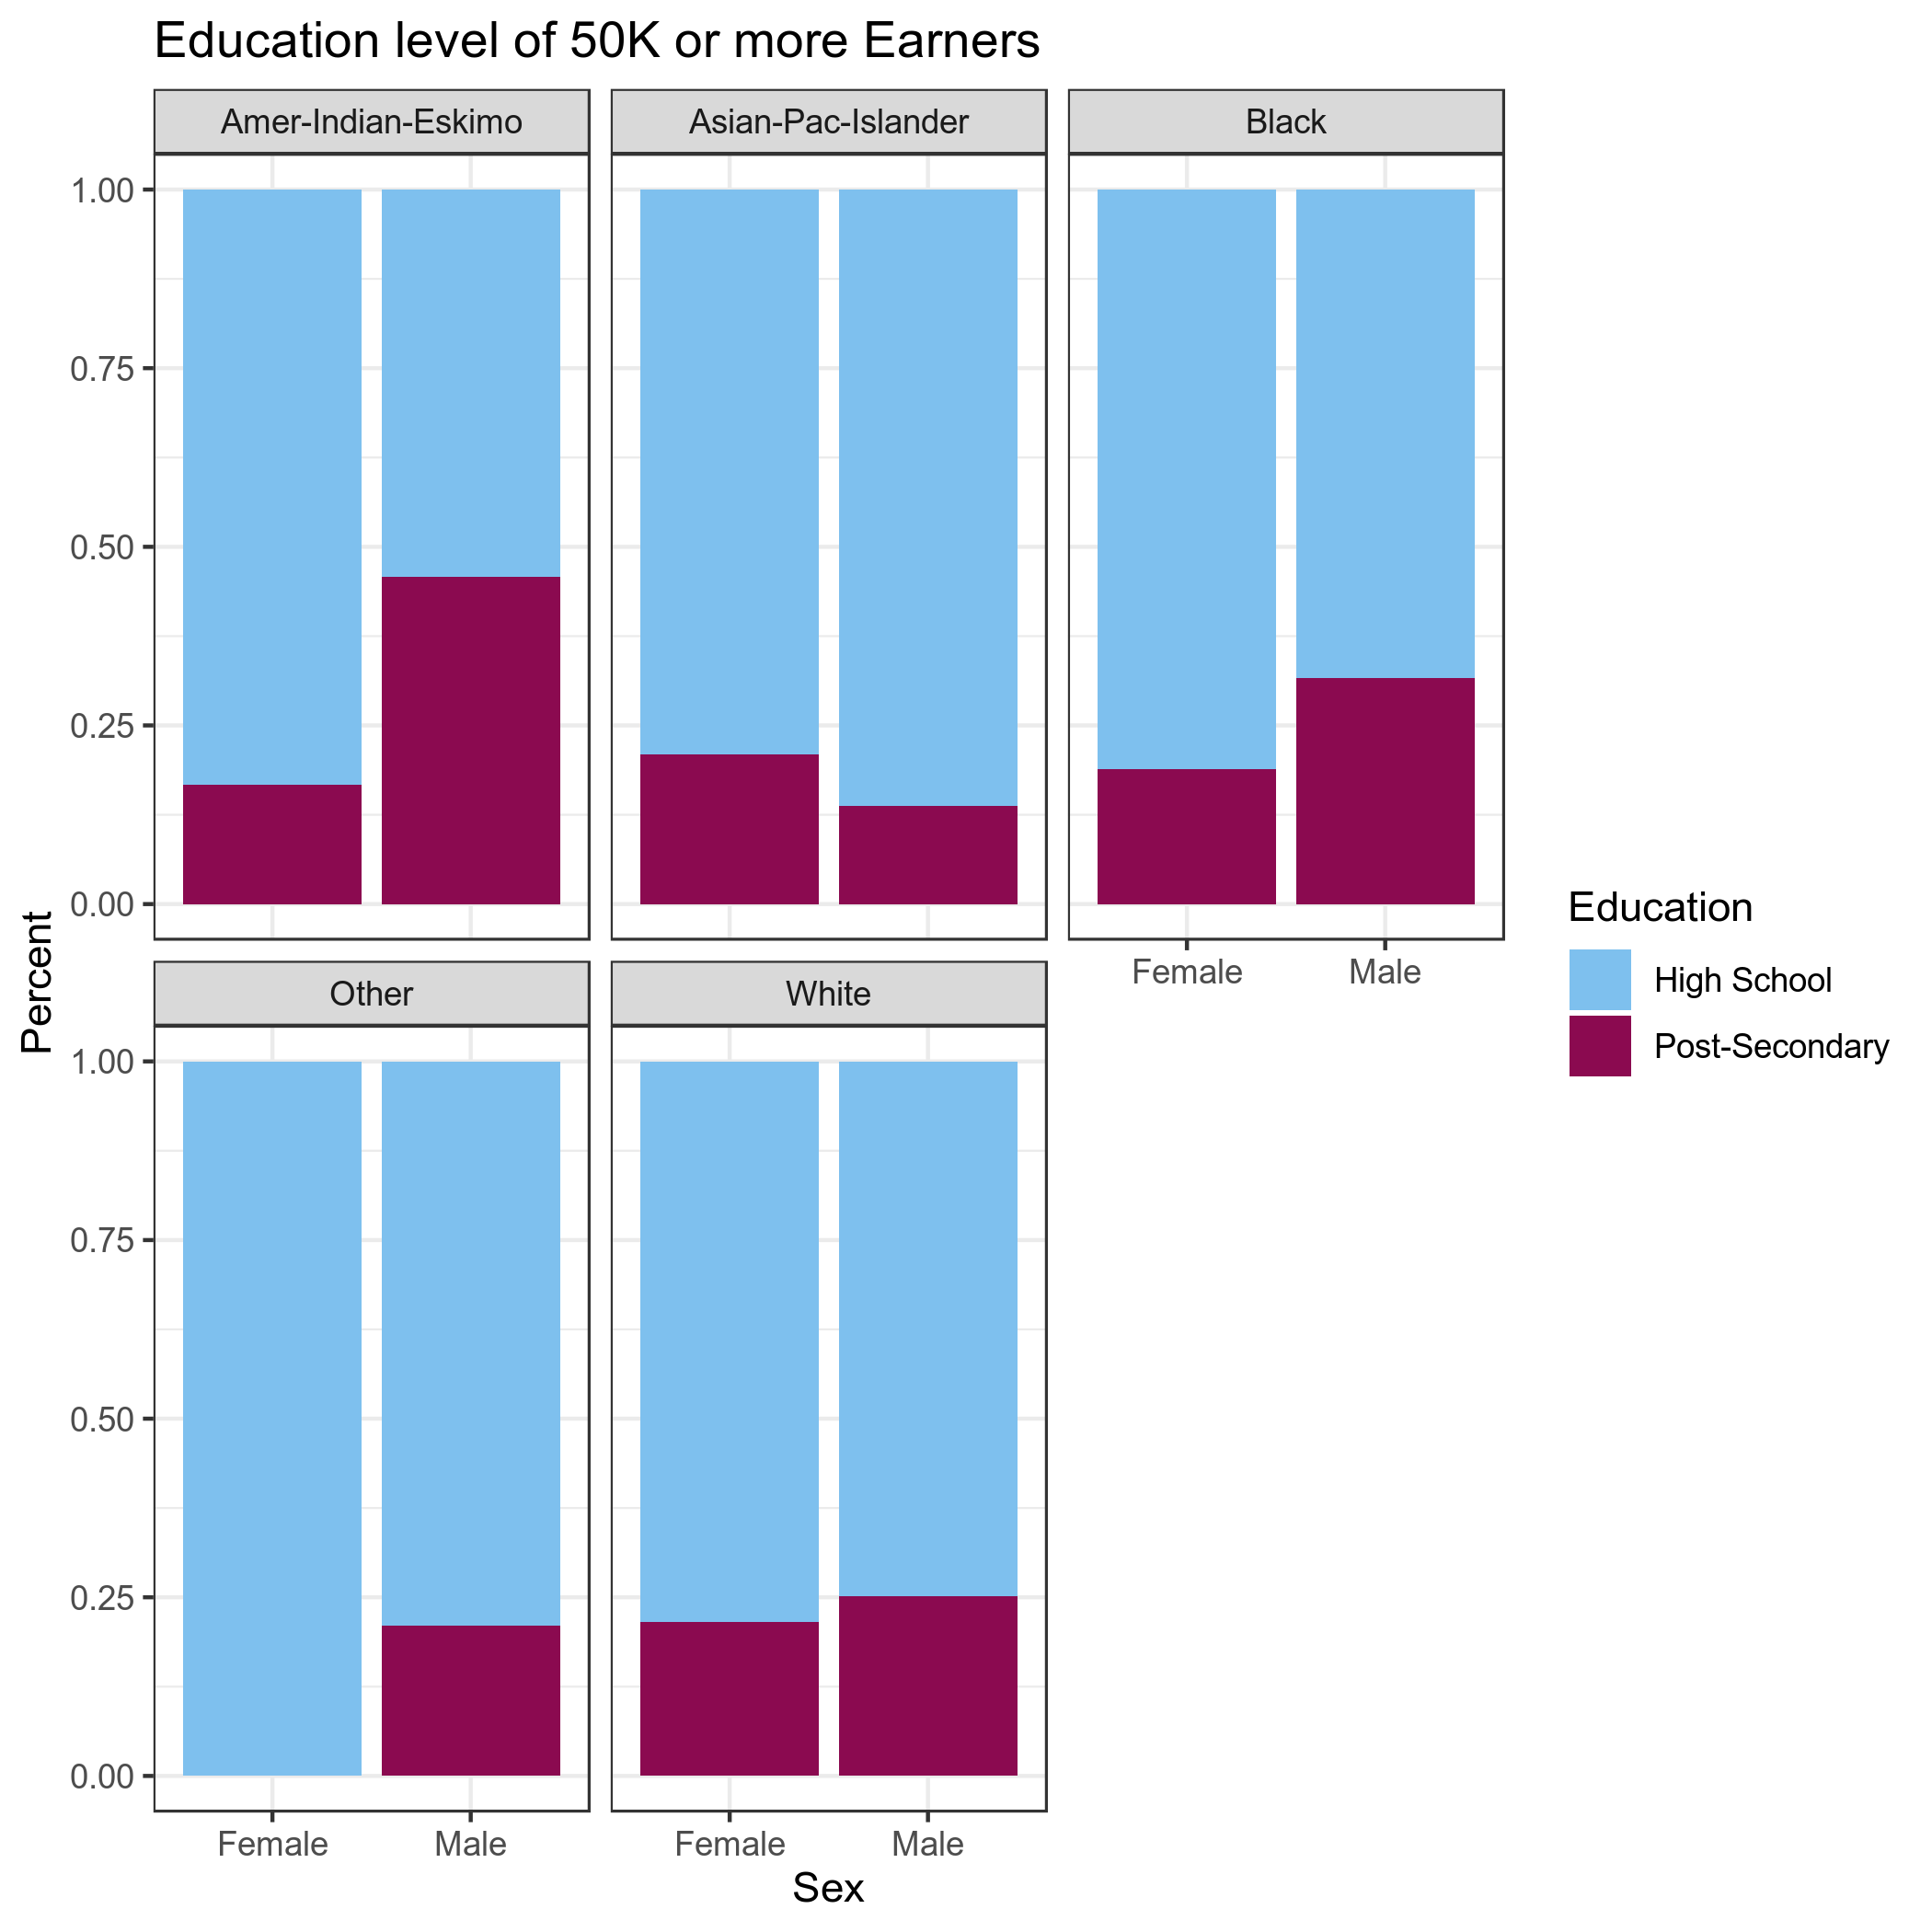
\includegraphics{../images/Plot_2_Education_Level_of_50K_or_more_Earners.png}

\hypertarget{number-of-work-hours-and-age}{%
\subsubsection{Number of Work Hours and
Age}\label{number-of-work-hours-and-age}}

We can deduce from the graph below that individuals work the most hours
between their 40's and 60's (probably full time at 40 hours or more a
week) and that employees under 20 and over 80 years of age work the same
number of hours (probably part time at 25 hours)

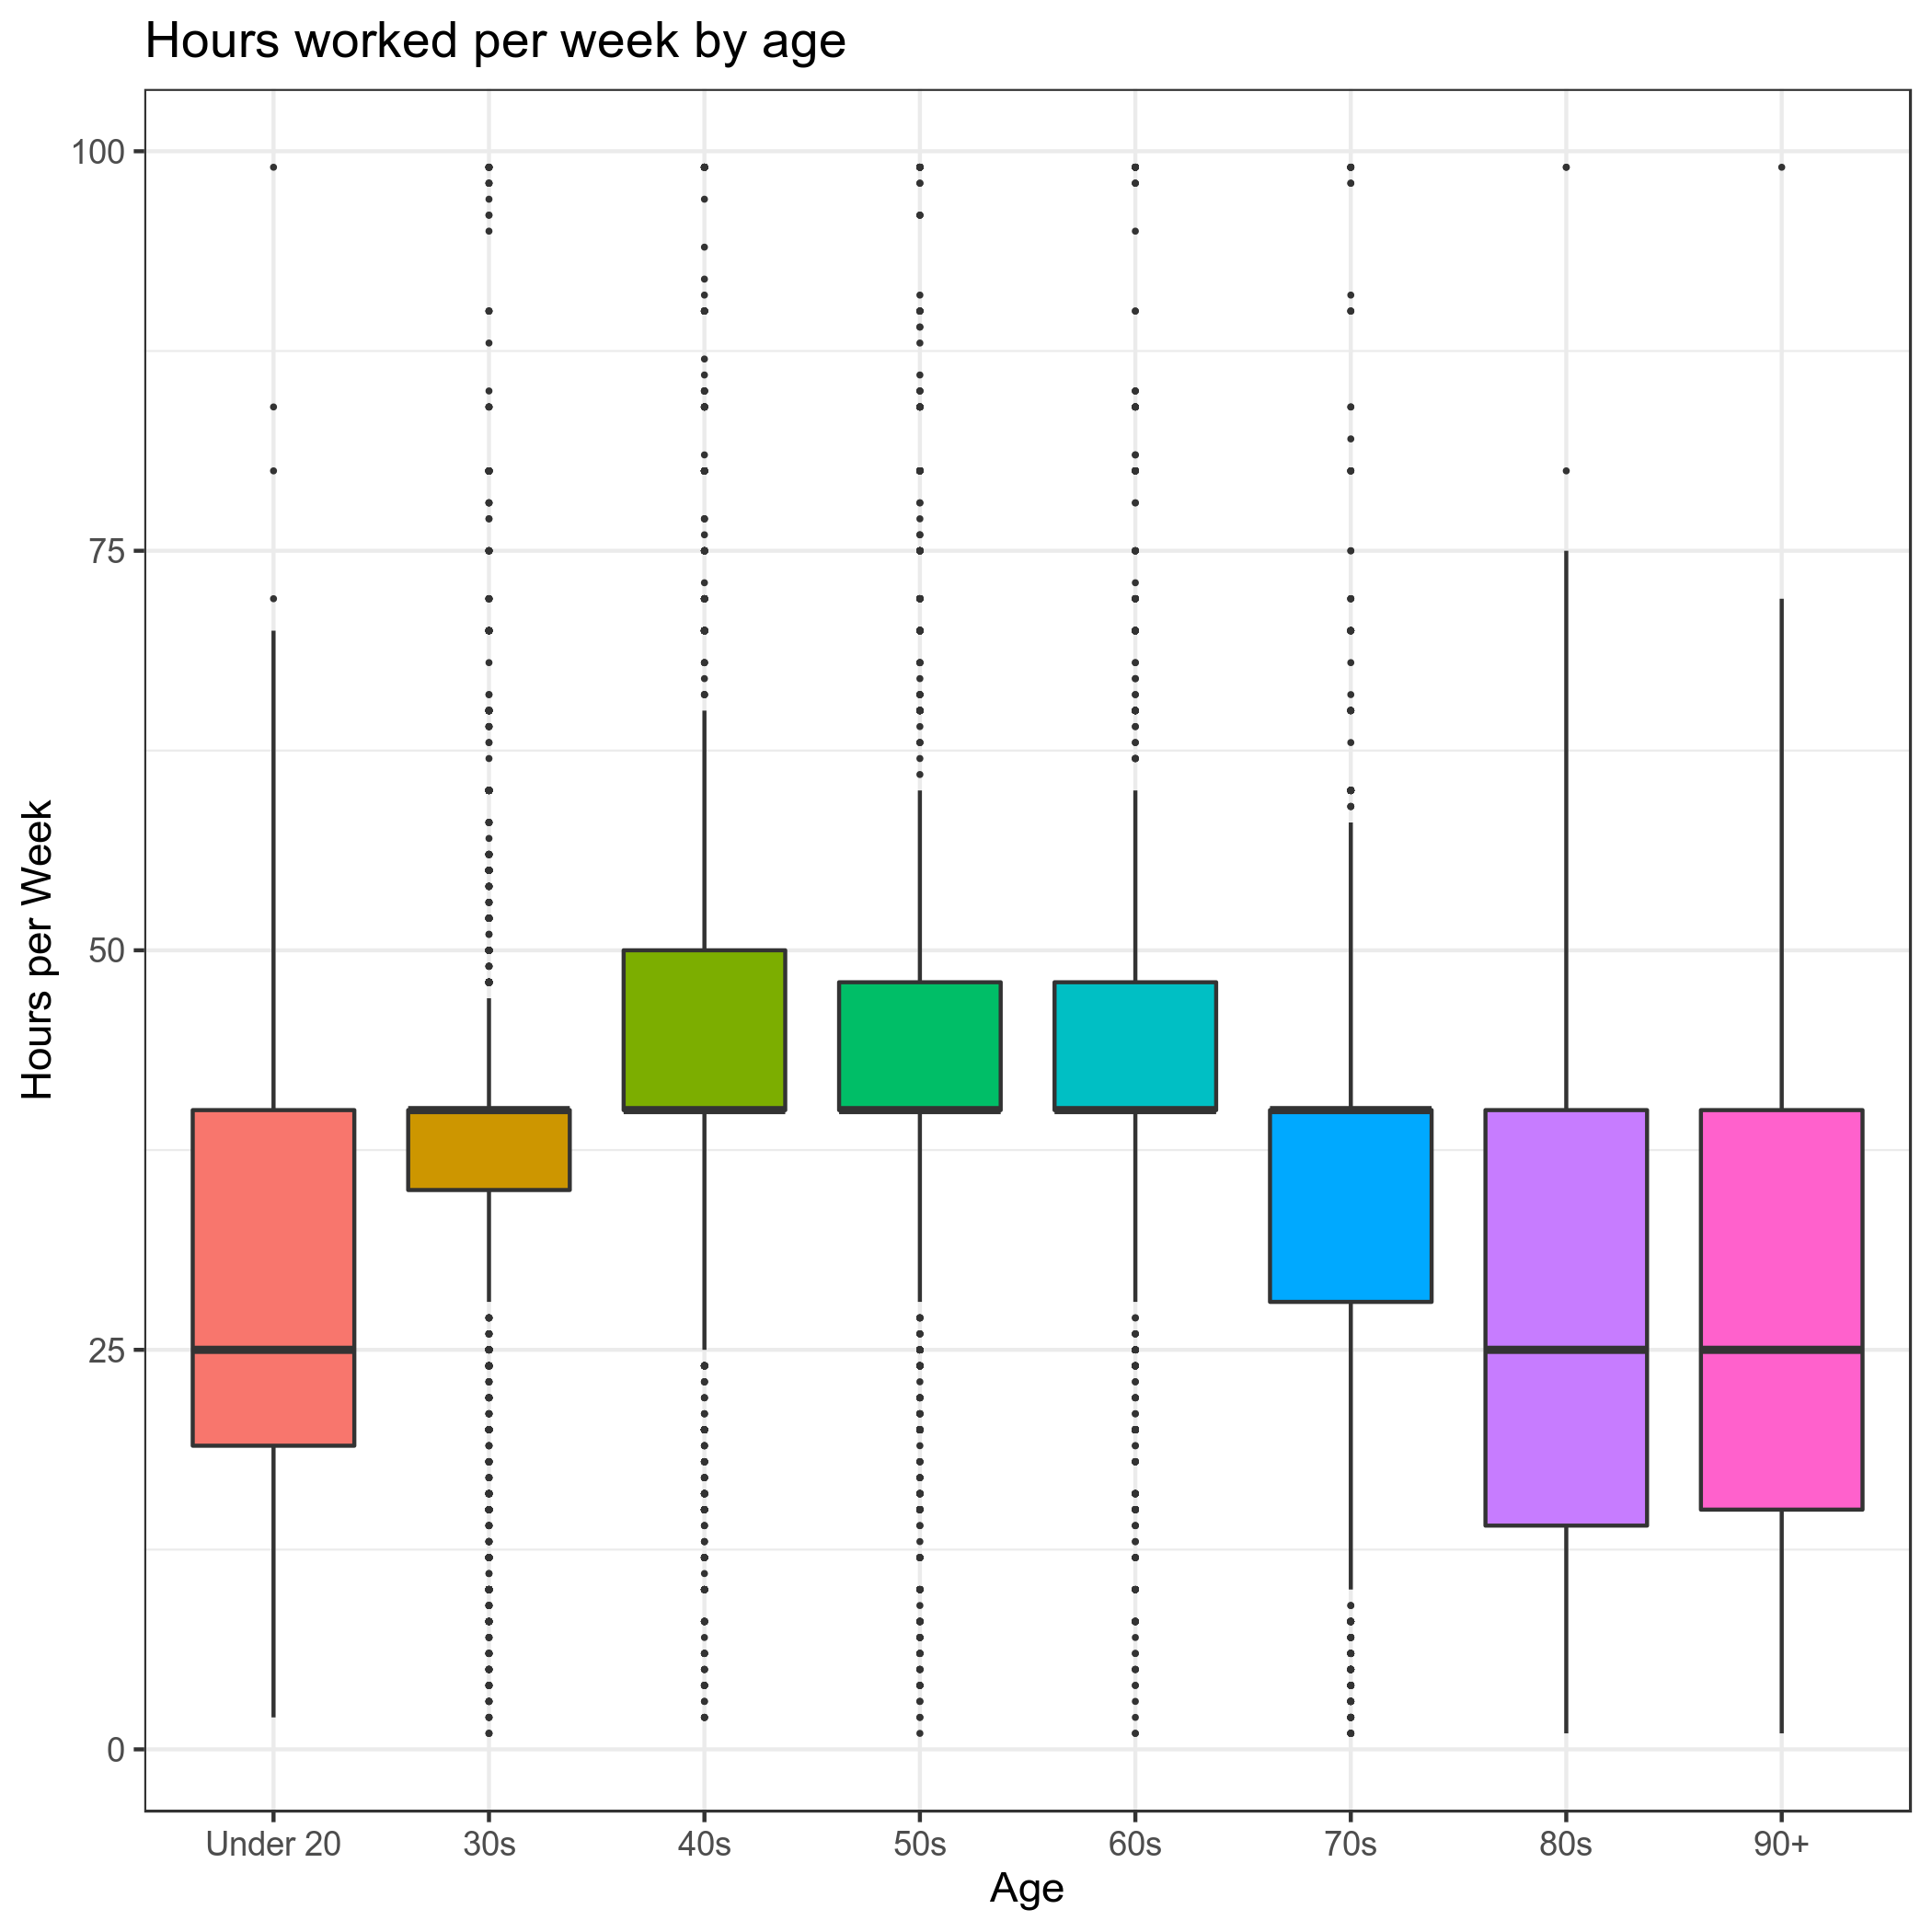
\includegraphics{../images/Plot_3_Hours_worked_per_week_by_age.png}

\hypertarget{marital-status-and-number-of-hours-worked}{%
\subsubsection{Marital Status and Number of Hours
Worked}\label{marital-status-and-number-of-hours-worked}}

The plot below shows that the working hours between married individuals
and single employees are similar.

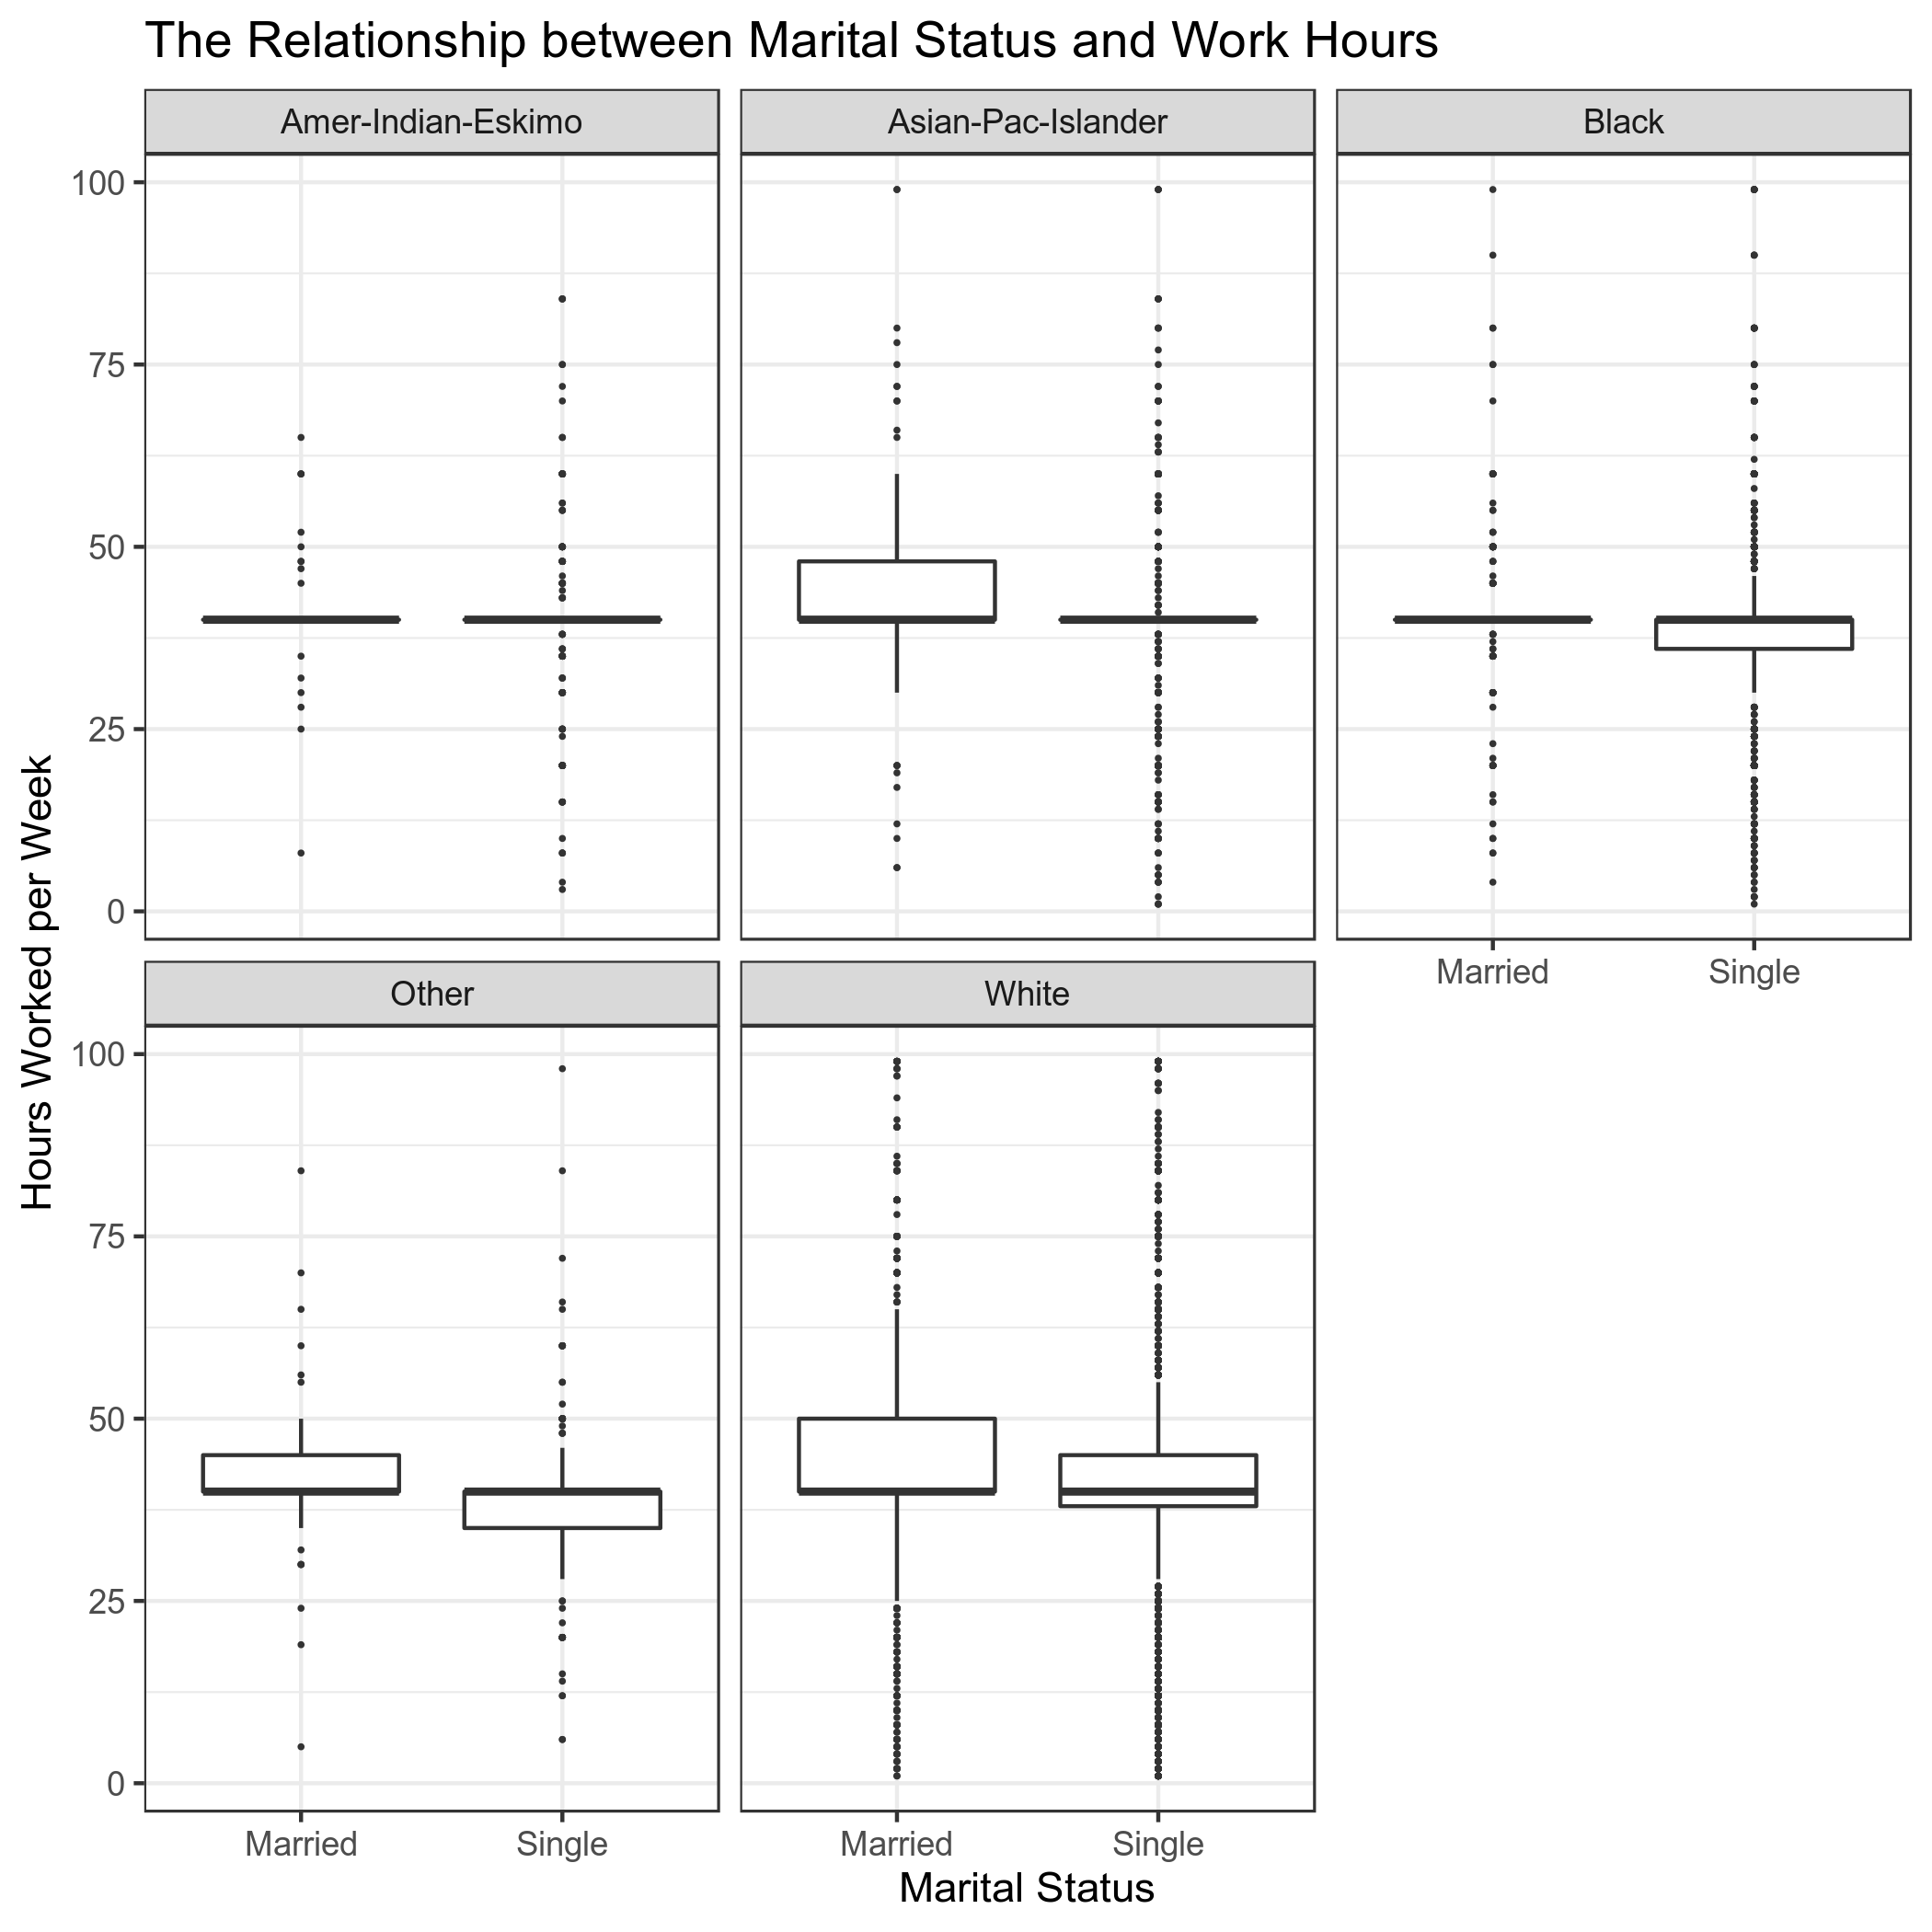
\includegraphics{../images/Plot_4_Marital_Status_and_Work_Hours.png}

\hypertarget{linear-regression}{%
\subsection{Linear Regression}\label{linear-regression}}

We have performed linear regression of hours per week vs.~each variable
separately, as well as linear regression using all these variables
together.

This was done using the lm function of the purrr package. For example:
lm(hours\_per\_week\textasciitilde{}education,data)

For categorical variables sex, education and relationship, the intercept
is the defaul reference group, where the ``estimate'' is the mean of
that group, and the ``estimates'' of all other variables are the
differences in means between that group and the reference. The statistic
is the t-statistic comparing these means, with a given p-value reporting
the significance of this difference.

\hypertarget{hypothesis-and-results}{%
\subsection{Hypothesis and Results}\label{hypothesis-and-results}}

\hypertarget{hours-vs.relationship}{%
\paragraph{Hours vs.~Relationship}\label{hours-vs.relationship}}

\textbf{Hypotheses:} Husbands work more than wives since wives are the
primary care takers of the household. Unmarried and individuals not in a
family work more than husbands or wives since they have more flexible
schedules and more time.

\textbf{Results:}

\begin{table}[H]
\centering
\begin{tabular}{l|r|r|r|r}
\hline
term & estimate & std.error & statistic & p.value\\
\hline
(Intercept) & 32.8759172 & 0.7907375 & 41.5762726 & 0.0000000\\
\hline
sexMale & 5.6914173 & 0.1409826 & 40.3696318 & 0.0000000\\
\hline
education11th & -2.7257409 & 0.5182506 & -5.2595035 & 0.0000001\\
\hline
education12th & -1.0448088 & 0.6870782 & -1.5206548 & 0.1283562\\
\hline
education1st-4th & 0.7558463 & 0.9908270 & 0.7628439 & 0.4455620\\
\hline
education5th-6th & 1.3619671 & 0.7546659 & 1.8047286 & 0.0711264\\
\hline
education7th-8th & 1.6580749 & 0.6068782 & 2.7321377 & 0.0062959\\
\hline
education9th & 0.7338944 & 0.6487072 & 1.1313184 & 0.2579294\\
\hline
educationAssoc-acdm & 3.8926669 & 0.5293446 & 7.3537487 & 0.0000000\\
\hline
educationAssoc-voc & 4.7743509 & 0.5004699 & 9.5397370 & 0.0000000\\
\hline
educationBachelors & 5.4530816 & 0.4195405 & 12.9977493 & 0.0000000\\
\hline
educationDoctorate & 9.0819689 & 0.7002813 & 12.9690303 & 0.0000000\\
\hline
educationHS-grad & 3.5205013 & 0.4033969 & 8.7271411 & 0.0000000\\
\hline
educationMasters & 6.6058589 & 0.4816350 & 13.7154871 & 0.0000000\\
\hline
educationPreschool & -0.4435165 & 1.6982491 & -0.2611610 & 0.7939700\\
\hline
educationProf-school & 9.3256894 & 0.6276622 & 14.8578147 & 0.0000000\\
\hline
educationSome-college & 2.2215778 & 0.4107771 & 5.4082322 & 0.0000001\\
\hline
age & 0.0213773 & 0.0049447 & 4.3232474 & 0.0000154\\
\hline
raceAsian-Pac-Islander & -1.5191519 & 0.7649342 & -1.9859904 & 0.0470428\\
\hline
raceBlack & -1.0175832 & 0.7022498 & -1.4490330 & 0.1473380\\
\hline
raceOther & -0.2743632 & 0.9823649 & -0.2792885 & 0.7800252\\
\hline
raceWhite & -0.4243259 & 0.6736736 & -0.6298686 & 0.5287850\\
\hline
\end{tabular}
\end{table}

In this case, we are comparing the mean hours worked per week of
husbands (intercept) to each other relationship category. It appears
that husbands work more than any other age group, (as seen by the
negative estimates), with significant p-values in each case.

\begin{Shaded}
\begin{Highlighting}[]
\KeywordTok{tidy}\NormalTok{(test_relationship)}\OperatorTok{$}\NormalTok{p.value}
\end{Highlighting}
\end{Shaded}

\begin{verbatim}
## [1] NA  0
\end{verbatim}

Comparing the full model to the model with no relationship info, we can
see that relationship does have a significant effect on hours worked per
week, with a p value of near 0

\hypertarget{hours-vs.sex}{%
\paragraph{Hours vs.~Sex}\label{hours-vs.sex}}

\textbf{Hypothesis:} Males work more hours than women given that women
tend to be the care takers of the household.

\textbf{Results:}

\begin{table}[H]
\centering
\begin{tabular}{l|r|r|r|r}
\hline
term & estimate & std.error & statistic & p.value\\
\hline
(Intercept) & 45.6847692 & 0.7930243 & 57.6082831 & 0.0000000\\
\hline
education11th & -2.3984193 & 0.5081966 & -4.7194713 & 0.0000024\\
\hline
education12th & -0.4493082 & 0.6736749 & -0.6669511 & 0.5048081\\
\hline
education1st-4th & 0.3616861 & 0.9716930 & 0.3722226 & 0.7097295\\
\hline
education5th-6th & 0.6912154 & 0.7407410 & 0.9331405 & 0.3507544\\
\hline
education7th-8th & 1.3344826 & 0.5950201 & 2.2427521 & 0.0249195\\
\hline
education9th & 0.5613643 & 0.6360024 & 0.8826449 & 0.3774347\\
\hline
educationAssoc-acdm & 2.5004900 & 0.5196590 & 4.8117899 & 0.0000015\\
\hline
educationAssoc-voc & 3.2416635 & 0.4914013 & 6.5967743 & 0.0000000\\
\hline
educationBachelors & 4.0753888 & 0.4125985 & 9.8773712 & 0.0000000\\
\hline
educationDoctorate & 7.8066512 & 0.6872874 & 11.3586416 & 0.0000000\\
\hline
educationHS-grad & 2.6605696 & 0.3958275 & 6.7215385 & 0.0000000\\
\hline
educationMasters & 5.0364866 & 0.4733910 & 10.6391693 & 0.0000000\\
\hline
educationPreschool & -0.3712434 & 1.6652630 & -0.2229338 & 0.8235884\\
\hline
educationProf-school & 7.9281041 & 0.6165185 & 12.8594741 & 0.0000000\\
\hline
educationSome-college & 1.5559376 & 0.4026910 & 3.8638500 & 0.0001118\\
\hline
relationshipNot-in-family & -3.8350001 & 0.1653245 & -23.1968057 & 0.0000000\\
\hline
relationshipOther-relative & -7.0112068 & 0.3910806 & -17.9277783 & 0.0000000\\
\hline
relationshipOwn-child & -11.4675017 & 0.2197320 & -52.1885755 & 0.0000000\\
\hline
relationshipUnmarried & -4.6884233 & 0.2265413 & -20.6956670 & 0.0000000\\
\hline
relationshipWife & -7.5408837 & 0.3102768 & -24.3037324 & 0.0000000\\
\hline
age & -0.0898299 & 0.0054207 & -16.5715434 & 0.0000000\\
\hline
raceAsian-Pac-Islander & -1.1430075 & 0.7503539 & -1.5232913 & 0.1276956\\
\hline
raceBlack & -1.0699053 & 0.6884585 & -1.5540594 & 0.1201800\\
\hline
raceOther & -0.8383543 & 0.9632921 & -0.8703013 & 0.3841422\\
\hline
raceWhite & -0.4155536 & 0.6607437 & -0.6289180 & 0.5294071\\
\hline
\end{tabular}
\end{table}

From this output, we can see that the average hours worked per week for
women is 45.7, and men work -2 hours per week on average compared to
women.

\begin{Shaded}
\begin{Highlighting}[]
\KeywordTok{tidy}\NormalTok{(test_sex)}\OperatorTok{$}\NormalTok{p.value}
\end{Highlighting}
\end{Shaded}

\begin{verbatim}
## [1]            NA 9.079086e-112
\end{verbatim}

Comparing the full model to the model with no sex info, we can see that
sex does have a significant effect on hours worked per week, with a p
value of \ensuremath{9.0790857\times 10^{-112}}

\hypertarget{hours-vs.age}{%
\paragraph{Hours vs.~Age}\label{hours-vs.age}}

\textbf{Hypothesis:} Individuals start to increase work hours in their
20s as they begin a career and keep increasing or plateauing depending
on their marital status until it declines at retirement (around 60 years
old).

\textbf{Results:}

\begin{table}[H]
\centering
\begin{tabular}{l|r|r|r|r}
\hline
term & estimate & std.error & statistic & p.value\\
\hline
(Intercept) & 37.3192009 & 0.7785095 & 47.9367341 & 0.0000000\\
\hline
sexMale & 4.2170727 & 0.1788891 & 23.5736657 & 0.0000000\\
\hline
education11th & -2.0089308 & 0.5057768 & -3.9719714 & 0.0000714\\
\hline
education12th & -0.2536480 & 0.6705897 & -0.3782461 & 0.7052502\\
\hline
education1st-4th & -0.2175083 & 0.9669353 & -0.2249461 & 0.8220226\\
\hline
education5th-6th & 0.3365756 & 0.7374331 & 0.4564152 & 0.6480945\\
\hline
education7th-8th & 0.6722287 & 0.5908766 & 1.1376803 & 0.2552624\\
\hline
education9th & 0.2632590 & 0.6331903 & 0.4157660 & 0.6775840\\
\hline
educationAssoc-acdm & 2.9399743 & 0.5174695 & 5.6814448 & 0.0000000\\
\hline
educationAssoc-voc & 3.6576562 & 0.4894155 & 7.4735197 & 0.0000000\\
\hline
educationBachelors & 4.3550053 & 0.4108797 & 10.5992232 & 0.0000000\\
\hline
educationDoctorate & 7.4759528 & 0.6837033 & 10.9344992 & 0.0000000\\
\hline
educationHS-grad & 2.7976545 & 0.3941757 & 7.0974815 & 0.0000000\\
\hline
educationMasters & 5.0747684 & 0.4712905 & 10.7678134 & 0.0000000\\
\hline
educationPreschool & -0.8808143 & 1.6579873 & -0.5312551 & 0.5952456\\
\hline
educationProf-school & 7.7337464 & 0.6137148 & 12.6015316 & 0.0000000\\
\hline
educationSome-college & 2.0141630 & 0.4010475 & 5.0222553 & 0.0000005\\
\hline
relationshipNot-in-family & -1.4155647 & 0.1821146 & -7.7729350 & 0.0000000\\
\hline
relationshipOther-relative & -4.2085729 & 0.3933235 & -10.7000291 & 0.0000000\\
\hline
relationshipOwn-child & -7.9905463 & 0.2110469 & -37.8614647 & 0.0000000\\
\hline
relationshipUnmarried & -1.1775836 & 0.2630903 & -4.4759670 & 0.0000076\\
\hline
relationshipWife & -3.0150898 & 0.3559552 & -8.4704199 & 0.0000000\\
\hline
raceAsian-Pac-Islander & -1.0890407 & 0.7471663 & -1.4575614 & 0.1449711\\
\hline
raceBlack & -0.9109186 & 0.6855929 & -1.3286582 & 0.1839701\\
\hline
raceOther & -0.2734727 & 0.9589600 & -0.2851764 & 0.7755108\\
\hline
raceWhite & -0.4001590 & 0.6579254 & -0.6082134 & 0.5430502\\
\hline
\end{tabular}
\end{table}

\begin{Shaded}
\begin{Highlighting}[]
\KeywordTok{tidy}\NormalTok{(test_age)}\OperatorTok{$}\NormalTok{p.value}
\end{Highlighting}
\end{Shaded}

\begin{verbatim}
## [1]           NA 2.507908e-51
\end{verbatim}

Comparing the full model to the model with no age info, we can see that
age does have a significant effect on hours worked per week, with a p
value of \ensuremath{2.507908\times 10^{-51}}

\hypertarget{hours-vs.education}{%
\paragraph{Hours vs.~Education}\label{hours-vs.education}}

\textbf{Hypothesis:} Higher educational attainment provides job security
and stability leading to more work hours for higher educated
individuals.

\textbf{Results:}

\begin{table}[H]
\centering
\begin{tabular}{l|r|r|r|r}
\hline
term & estimate & std.error & statistic & p.value\\
\hline
(Intercept) & 43.3263038 & 0.7316320 & 59.2187075 & 0.0000000\\
\hline
sexMale & 3.9614292 & 0.1802404 & 21.9785823 & 0.0000000\\
\hline
relationshipNot-in-family & -2.0367467 & 0.1864589 & -10.9233023 & 0.0000000\\
\hline
relationshipOther-relative & -6.0376017 & 0.3987168 & -15.1425807 & 0.0000000\\
\hline
relationshipOwn-child & -10.4381682 & 0.2340288 & -44.6020621 & 0.0000000\\
\hline
relationshipUnmarried & -2.0769597 & 0.2655478 & -7.8214151 & 0.0000000\\
\hline
relationshipWife & -3.5494329 & 0.3599806 & -9.8600676 & 0.0000000\\
\hline
age & -0.0733219 & 0.0053728 & -13.6467450 & 0.0000000\\
\hline
raceAsian-Pac-Islander & -0.0221594 & 0.7510028 & -0.0295064 & 0.9764609\\
\hline
raceBlack & -0.7379608 & 0.6907118 & -1.0684062 & 0.2853452\\
\hline
raceOther & -0.6818600 & 0.9654061 & -0.7062935 & 0.4800107\\
\hline
raceWhite & 0.0971549 & 0.6625748 & 0.1466323 & 0.8834231\\
\hline
\end{tabular}
\end{table}

In this analysis, the default reference group (intercept) is a 10th
grade education. It appears that those with an 11th grade education work
3.96 hours less (significant p-value), whereas all other with no more
than a high school education work the same amount (no significant
p-values).

Every other education level higher than high school worked significantly
more hours, as seen by positive estimates of each group and low
p-values.

\begin{Shaded}
\begin{Highlighting}[]
\KeywordTok{tidy}\NormalTok{(test_education)}\OperatorTok{$}\NormalTok{p.value}
\end{Highlighting}
\end{Shaded}

\begin{verbatim}
## [1]            NA 1.039446e-148
\end{verbatim}

Comparing the full model to the model with no education info, we can see
that education does have a significant effect on hours worked per week,
with a p value of \ensuremath{1.0394462\times 10^{-148}}

\hypertarget{hours-vs.race}{%
\paragraph{Hours vs.~Race}\label{hours-vs.race}}

\textbf{Hypothesis:} Race does not have a correlation with hours worked
since legal work hours required are not based on race but more on the
other factors previously explored.

\textbf{Results:}

\begin{table}[H]
\centering
\begin{tabular}{l|r|r|r|r}
\hline
term & estimate & std.error & statistic & p.value\\
\hline
(Intercept) & 40.6273698 & 0.4958668 & 81.9320153 & 0.0000000\\
\hline
sexMale & 4.0438025 & 0.1785923 & 22.6426434 & 0.0000000\\
\hline
education11th & -2.2620467 & 0.5043212 & -4.4853295 & 0.0000073\\
\hline
education12th & -0.5355350 & 0.6683341 & -0.8012982 & 0.4229649\\
\hline
education1st-4th & 0.3053957 & 0.9636848 & 0.3169041 & 0.7513184\\
\hline
education5th-6th & 0.5750503 & 0.7344659 & 0.7829503 & 0.4336620\\
\hline
education7th-8th & 1.3423145 & 0.5902245 & 2.2742439 & 0.0229578\\
\hline
education9th & 0.4297094 & 0.6310903 & 0.6809000 & 0.4959396\\
\hline
educationAssoc-acdm & 2.7780743 & 0.5156767 & 5.3872400 & 0.0000001\\
\hline
educationAssoc-voc & 3.5512186 & 0.4876001 & 7.2830553 & 0.0000000\\
\hline
educationBachelors & 4.2592346 & 0.4088867 & 10.4166632 & 0.0000000\\
\hline
educationDoctorate & 7.9350595 & 0.6814153 & 11.6449681 & 0.0000000\\
\hline
educationHS-grad & 2.7842538 & 0.3927560 & 7.0890158 & 0.0000000\\
\hline
educationMasters & 5.2975034 & 0.4692626 & 11.2889963 & 0.0000000\\
\hline
educationPreschool & -0.5669836 & 1.6519409 & -0.3432227 & 0.7314331\\
\hline
educationProf-school & 7.9516931 & 0.6110522 & 13.0131153 & 0.0000000\\
\hline
educationSome-college & 1.8576814 & 0.3996749 & 4.6479814 & 0.0000034\\
\hline
relationshipNot-in-family & -1.9376733 & 0.1844416 & -10.5056209 & 0.0000000\\
\hline
relationshipOther-relative & -5.2350263 & 0.3954076 & -13.2395685 & 0.0000000\\
\hline
relationshipOwn-child & -9.5673730 & 0.2339261 & -40.8991236 & 0.0000000\\
\hline
relationshipUnmarried & -1.6529304 & 0.2615099 & -6.3207191 & 0.0000000\\
\hline
relationshipWife & -3.5196793 & 0.3561062 & -9.8837909 & 0.0000000\\
\hline
age & -0.0813743 & 0.0053874 & -15.1044823 & 0.0000000\\
\hline
\end{tabular}
\end{table}

\begin{Shaded}
\begin{Highlighting}[]
\KeywordTok{tidy}\NormalTok{(test_race)}\OperatorTok{$}\NormalTok{p.value}
\end{Highlighting}
\end{Shaded}

\begin{verbatim}
## [1]         NA 0.06580715
\end{verbatim}

Comparing the full model to the model with no race info, race does
\emph{not} have a significant effect on hours worked per week, with a p
value of 0.0658072

\hypertarget{discussion}{%
\subsection{Discussion}\label{discussion}}

Our data is quite biased in that there are much more men (21790) than
women (10771) in data set. This is especially apparent at older ages,
for instance there are 742 women over 60 and 1590 men over 60.

\hypertarget{conclusion}{%
\subsection{Conclusion}\label{conclusion}}

Education, age, sex and relationship all have a very significant effect
on the number of hours worked per week, while race does not.

\end{document}
